\section{Верификация}
% \subsection{Гипотеза о близости решений}
В литературе представлены \cite{borisov, formalskii, ZobovaTatarinovPMM} работы, рассматривающие омниколеса в предположении, что массой и инерцией роликов можно пренебречь, налагающие на систему неголономные связи, ограничивающие направление скорости скольжения в точках контакта колес с поверхностью, на которой стоит экипаж, и не вводящие силу трения в контакте, т.е. считающие скольжение идеальным. Эти идеализированные модели имеют существенно меньше степеней свободы, чем "реальный" омниэкипаж, и легче поддаются аналитическому исследованию.\\

Описанные модели можно использовать для верификации построенной физически-ориентированной модели, рассматривая некоторые элементарные виды движений. Максимальное соответствие построенной модели упомянутым неголономным может быть достигнуто при уменьшении вляиния массы роликов на динамику колеса, а именно, при уменьшении их массы с сохранением общей массы колеса с роликами. На этом предположении и основан наш подход к верификации.\\

\subsection{Проверочная модель}

Для верификации использованы результаты работы \cite{borisov} как новейшей из неголономных моделей динамики свободной тележки с омниколесами на плоскости.\\

Авторы \cite{borisov} принимают простейшую модель омниколеса как плоского диска, для которого скорость точки контакта с опорной поверхностью направлена вдоль прямой, составляющей некоторый угол $\delta$ с плоскостью колеса (см. рис.~\ref{fig:bor_wheel_scheme}). Связь, наложенная на колесо в таком случае имеет вид
$$\vec{v_Q}\cdot\vec{\alpha} = 0,$$
где $\vec{v_Q}$ - скорость точки контакта, $\vec{\alpha}$ - единичный вектор вдоль оси закрепления роликов.\\

\begin{figure}[ht!]
    \centering
    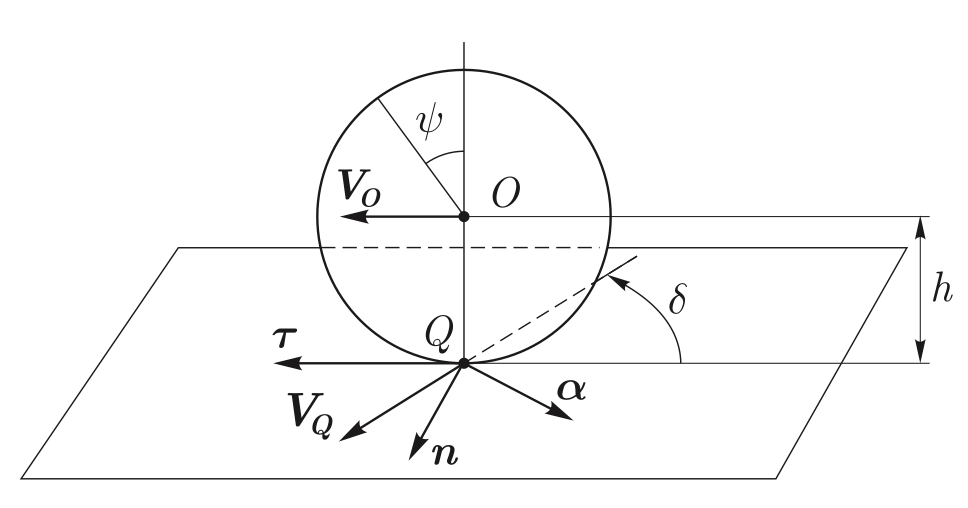
\includegraphics[width=0.75\textwidth]{content/parts/3_friction/diploma/img/art/bor_wheel_scheme.png}
    \caption{Неголономная модель колеса}
    \label{fig:bor_wheel_scheme}
\end{figure}

Авторы \cite{borisov} получают уравнения движения для экипажа с произвольным количеством колес, закрепленных так, что их оси неподвижны относительно платформы, а оси роликов повернуты на произвольные углы относительно плоскостей соответствующих колес (см.рис.~\ref{fig:bor_vehicle}).

\begin{figure}[ht!]
    \centering
    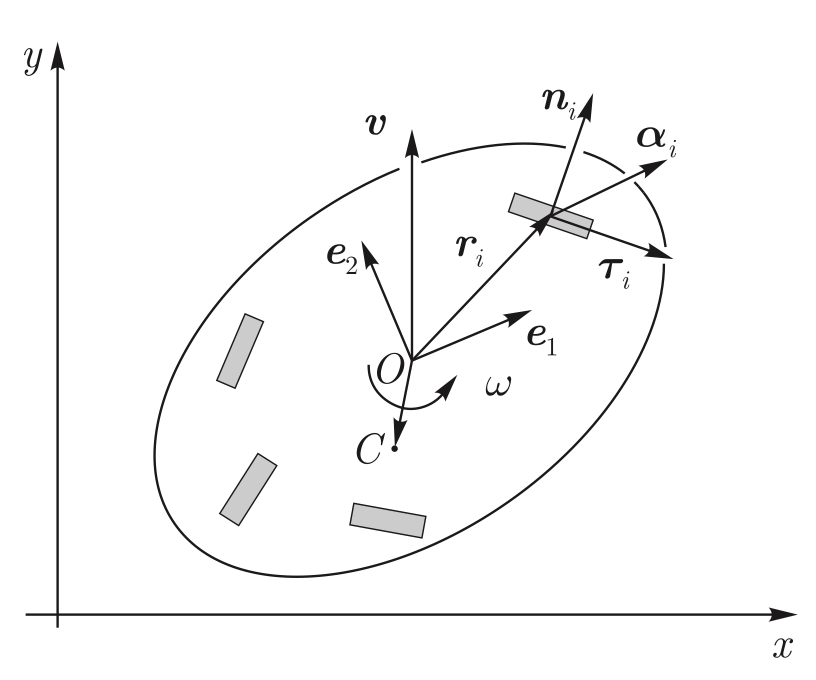
\includegraphics[width=0.75\textwidth]{content/parts/3_friction/diploma/img/art/bor_vehicle.png}
    \caption{Неголономная модель экипажа}
    \label{fig:bor_vehicle}
\end{figure}

Вводится подвижная система отсчета, связанная с платформой экипажа (см.рис.~\ref{fig:bor_vehicle}). Уравнения свободного движения имеют вид:
\begin{eqnarray*}
(\Gamma+mE)\dot{\vec{v}} + m\dot{\omega}(J\vec{r_C}+R)+m\omega J(\vec{v} + \omega J\vec{r_C}) = 0,\\
\hat{I}\dot{\omega} + m(J\vec{r_C}+\vec{r})\cdot\dot{\vec{v}}+m\omega\vec{v}\cdot\vec{r_C} = 0,\\
\dot{x} = v_1\cos\phi - v_2\sin\phi, \dot{x} = v_1\sin\phi + v_2\cos\phi, \dot{\phi} = \omega,\\
\Gamma_{kl} = \sum_i \frac{I_i}{s_i^2 h_i^2}\alpha_i^k\alpha_i^l, R = m^{-1}\sum_i \frac{I_i}{s_i^2 h_i^2}(J\vec{r_i}\cdot \alpha_i) \alpha_i,\\
\hat{I} = I + \sum_i \frac{I_i}{s_i^2 h_i}(J\vec{r_i}\cdot \alpha_i)^2,
\end{eqnarray*}%
\newline
где $\hat{I}$ - суммарный момент инерции системы относительно вертикальной оси, проходящей через начало $O$ подвижной системы отсчета,\newline
$I$ - момент инерции платформы относительно той же прямой,\newline
$I_i$ - моменты инерции колес относительно их диаметров,\newline
$s_i = \sin\delta_i$, $h_i$ - радиусы колес,\newline
$\vec{r_i}$ - точки закрепления осей колес в подвижной системе,\newline
$J = \left(\begin{array}{cc}0 & 1\\-1 & 0\end{array}\right)$,\newline
$x,y,\phi$ - координаты точки $O$ и угол поворота платвормы экипажа вокруг вертикальной оси,\newline
$\vec{v}, \omega$ - вектор скорости точки $O$ и скорость поворота платформы,\newline
$\vec{r_C}$ - координаты центра масс экипажа в подвижных осях,
$E$ - единичная матрица.\\

% Данная неголономная модель экипажа также реализована на языке Modelica \cite{ModelicaSpec} как часть упомянутой библиотеки \cite{KosenkoBond}. Таким образом, возможно проведение сравнительного анализа физически-ориентированной и идеализированной моделей и верифкация.


\subsection{Два типа движений}
Задавая параметры экипажа, такие как массы его частей, их моменты инерции, геометрические размеры, положения, а также начальные данные - скорость центра масс и угловую скорость платформы, - и выполняя согласованные расчеты для двух реализаций - физической и идеальной - можно получить достаточно близкие движения при достаточно малой доле массы роликов.\\

\begin{figure}[!ht]
    \centering
    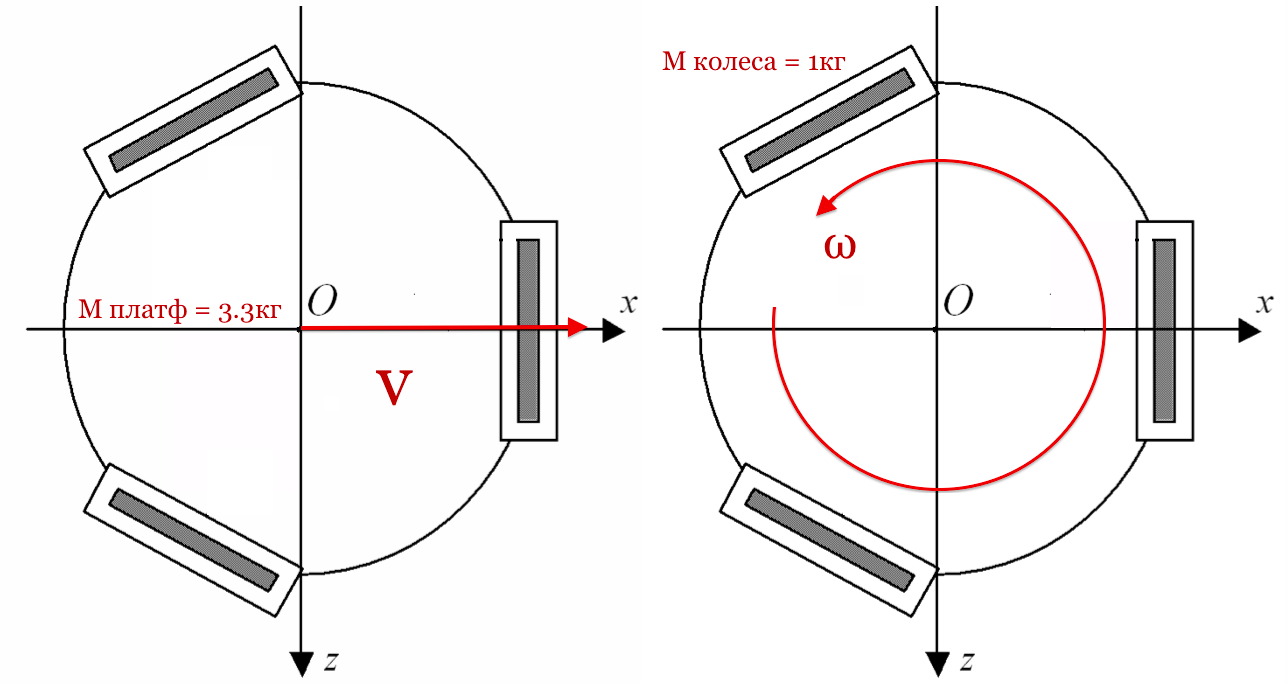
\includegraphics[width=0.95\textwidth]{content/parts/3_friction/diploma/img/art/my_exp_setup.png}
    \caption{Параметры экспериментов}
    \label{fig:my_exp_setup}
\end{figure}

При выполнении численных экспериментов массы платформы и колес, количество колес, количество роликов, геометрия системы были фиксированы (см. рис.~\ref{fig:my_exp_setup}). Изменялись начальные данные и доля массы роликов.\\

Рассмотрены два типа начальных условий $\vec{v}(0) = (v_0, 0, 0)^T, \omega(0) = \omega_0$ (см. рис.~\ref{fig:my_exp_setup}):
\begin{enumerate}
\item экипаж закручен вокруг вертикальной оси, проходящей через его центр масс, скорость центра масс равна нулю (ожидаемый результат - экипаж вращается вокруг своей вертикальной оси симметрии, и центр масс покоится),
\item экипаж имеет начальную линейную скорость в направлении одного из колес и не закручен (ожидаемый результат - центр масс экипажа движется вдоль оси $Ox$, экипаж не вращается).
\end{enumerate}

Значения отношения $\eta$ массы ролика к общей массе колеса принимали в обоих случаях значения от $10^{-6}n^{-1}$ до $10^{-1}n^{-1}$ с шагом $1$ по порядку малости (здесь $n$ - фиксированное количество роликов).

На рис.~\ref{fig:exp_examples} приведены примеры траектории центра масс $y(x)$ и зависимости $\psi(t)$ угла поворота $\psi$ платформы вокруг вертикальной оси, проходящей через её центр, для случаев 1) и 2). Кривые $y(x)$, изображающие траектории центра масс, соответствуют, в сущности, точке - началу координат - в случае $v_0 = 0, \omega_0 = 1$, и отрезку прямой, совпадающей с осью $x$, в случае $v_0 = 1, \omega_0 = 0$, ибо масштаб отображения таков, чтобы были видны отклонения от точных значений, возникающие в силу вычислительной погрешности, но сами эти отклонения имеют порядок малости, позволяющий считать их нулевыми. Аналогичное утверждение верно и для зависимости угла поворота платформы $\psi$ от времени в случае поступательного движения - полученная зависимость близка к постоянной.\\

Ниже представлены результаты нескольких численных экспериментов. Во всех случаях величины, изображенные на рис.~\ref{fig:exp_examples}, демонстрируют поведение, не различимое в масштабе рис.~\ref{fig:exp_examples}, и поэтому приведены лишь расхождения между построенной нами моделью и верификационной идеализацией, которые и представляют интерес. Также представлена абсолютная величина скорости скольжения в точке контакта в физической модели.\\

Графики зависимости скорости скольжения от времени показывают, что скольжение имеет место в окрестности момента смены роликов. Это объясняется тем, что для идеального качения в эти моменты ролику необходима бесконечная угловая скорость собственного вращения, ибо его размер вблизи вершины стремится к нулю. Видно, что с ростом доли массы роликов в общей массе колеса скольжение в контакте становится существеннее, изменяясь от пренебрежимо малого при $\eta = 10^{-6}$ до весьма существенного уже при $\eta = 10^{-3}$. Тем не менее, расхождения траектории и угла поворота платформы малы, а скольжение наблюдается лишь в точках колеса, которые в промышленных конструкциях не присутствуют (см. Обзор), что и позволяет считать верификацию проведенной.
\newpage

% EXAMPLES
\begin{figure}[h]
\centering
\begin{subfigure}{.47\textwidth}
    \centering
    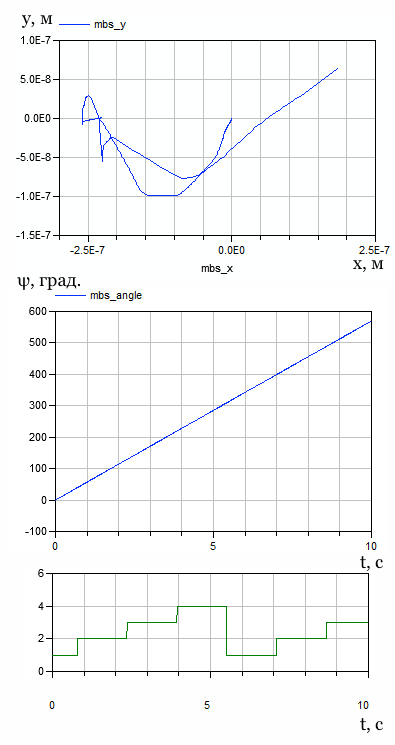
\includegraphics[width=\textwidth]{content/parts/3_friction/diploma/img/res/example_v_0_0_omega_1_frac_1e-1_n_4_time_10s.png}
    \caption{$\eta = 0,1, v_0 = 0, \omega_0 = 1$}
    \label{fig:exp_example_omega}
\end{subfigure}%
\hspace{5pt}
\begin{subfigure}{.47\textwidth}
    \centering
    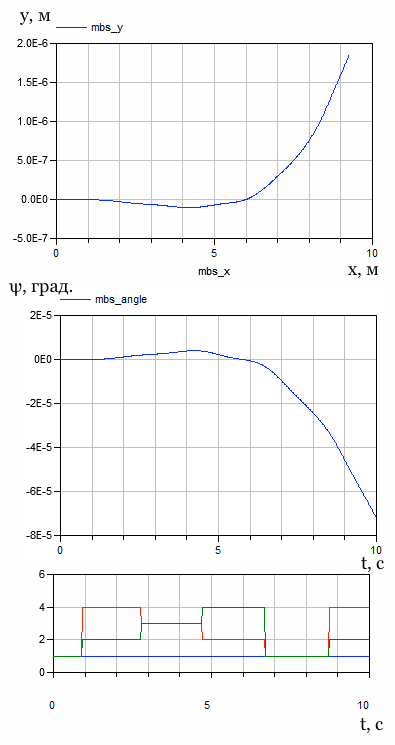
\includegraphics[width=\textwidth]{content/parts/3_friction/diploma/img/res/example_v_1_0_omega_0_frac_1e-1_n_4_time_10s.png}
    \caption{$\eta = 0,1, v_0 = 1, \omega_0 = 0$}
    \label{fig:exp_example_v}
\end{subfigure}
\caption{Примеры траекторий, характера изменения угла и смены номеров роликов в контакте для двух типов начальных условий. На нижнем графике - номер ролика в контакте, см. рис.~\ref{OmniWheel}}
\label{fig:exp_examples}
\end{figure}
\newpage

\begin{figure}[h]
\begin{center}\begin{equation*}\begin{array}{cc}
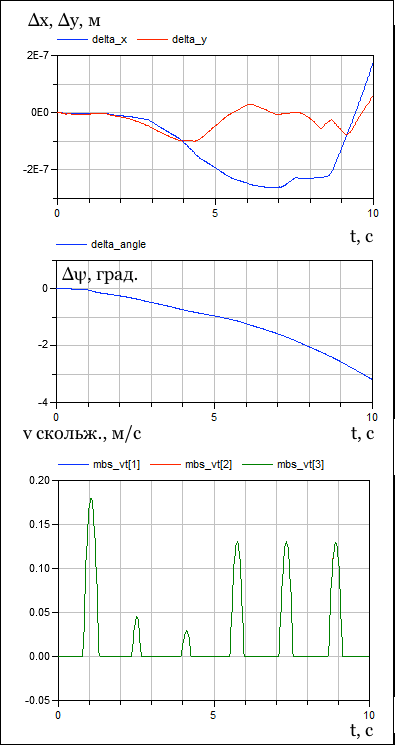
\includegraphics[width=7cm, viewport=0 0 395 745,clip]{content/parts/3_friction/diploma/img/res/comparison_v_0_0_omega_1_frac_1e-1_n_4_time_10s.png} & 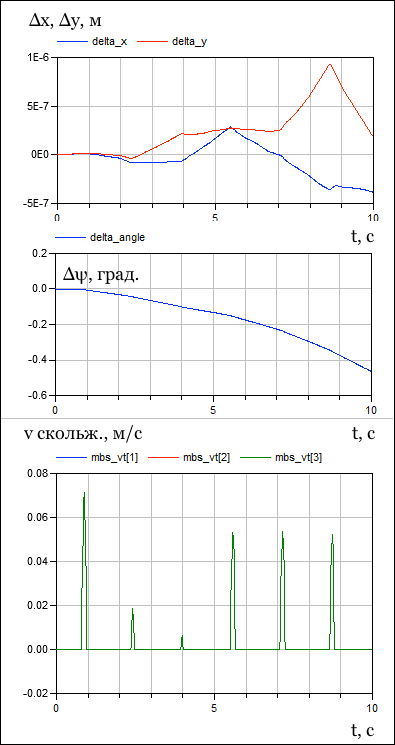
\includegraphics[width=7cm, viewport=0 0 395 745,clip]{content/parts/3_friction/diploma/img/res/comparison_v_0_0_omega_1_frac_1e-2_n_4_time_10s.png}\\
\eta = 0,1, v_0 = 0, \omega_0 = 1 & \eta = 0,01, v_0 = 0, \omega_0 = 1\\
\end{array}\end{equation*}\end{center}
\caption{Вращение экипажа с трением вокруг вертикальной оси}
\end{figure}
\newpage

\begin{figure}[h]
\begin{center}\begin{equation*}\begin{array}{cc}
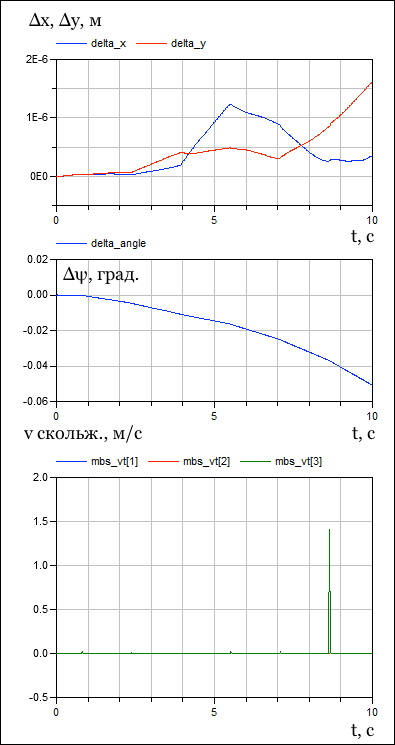
\includegraphics[width=7cm, viewport=0 0 395 745,clip]{content/parts/3_friction/diploma/img/res/comparison_v_0_0_omega_1_frac_1e-3_n_4_time_10s.png} & 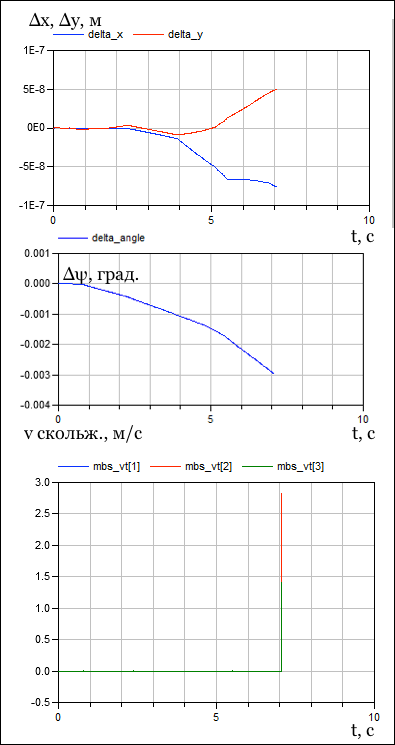
\includegraphics[width=7cm, viewport=0 0 395 745,clip]{content/parts/3_friction/diploma/img/res/comparison_v_0_0_omega_1_frac_1e-4_n_4_time_10s.png}\\
\eta = 0,001, v_0 = 0, \omega_0 = 1 & \eta = 0,0001, v_0 = 0, \omega_0 = 1\\
\end{array}\end{equation*}\end{center}
\caption{Вращение экипажа с трением вокруг вертикальной оси}
\end{figure}
\newpage

\begin{figure}[h]
\begin{center}\begin{equation*}\begin{array}{cc}
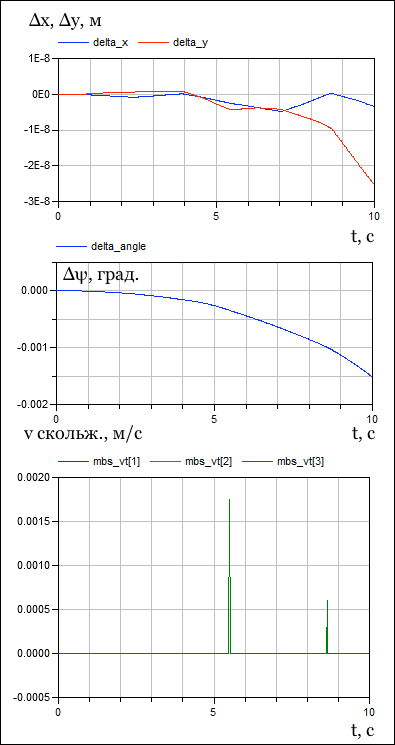
\includegraphics[width=7cm, viewport=0 0 395 745,clip]{content/parts/3_friction/diploma/img/res/comparison_v_0_0_omega_1_frac_1e-5_n_4_time_10s.png} & 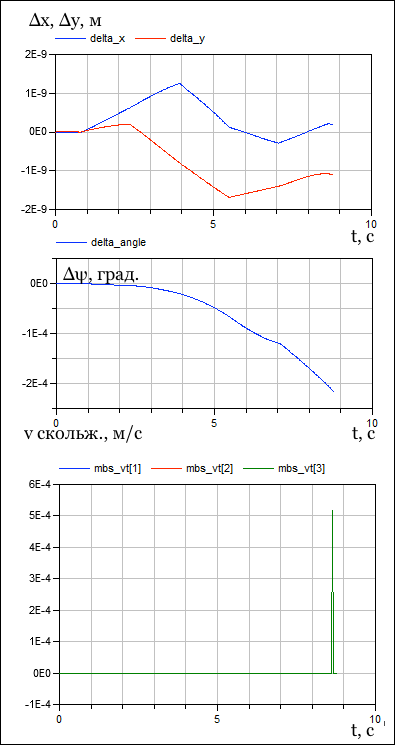
\includegraphics[width=7cm, viewport=0 0 395 745,clip]{content/parts/3_friction/diploma/img/res/comparison_v_0_0_omega_1_frac_1e-6_n_4_time_10s.png}\\
\eta = 10^{-5}, v_0 = 0, \omega_0 = 1 & \eta = 10^{-6}, v_0 = 0, \omega_0 = 1\\
\end{array}\end{equation*}\end{center}
\caption{Вращение экипажа с трением вокруг вертикальной оси}
\end{figure}
\newpage

\begin{figure}[h]
\begin{center}\begin{equation*}\begin{array}{cc}
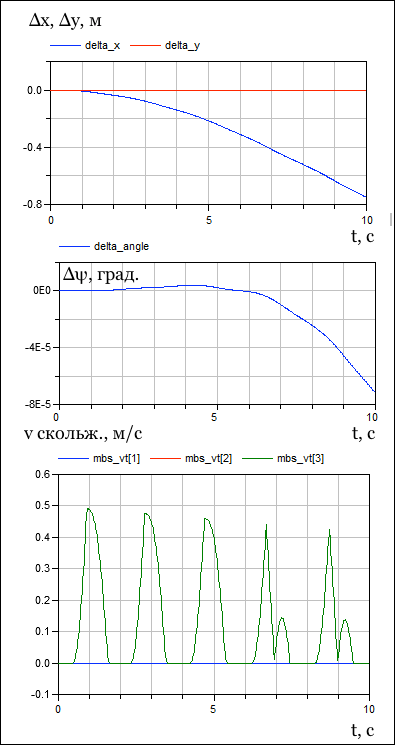
\includegraphics[width=7cm, viewport=0 0 395 745,clip]{content/parts/3_friction/diploma/img/res/comparison_v_1_0_omega_0_frac_1e-1_n_4_time_10s.png} & 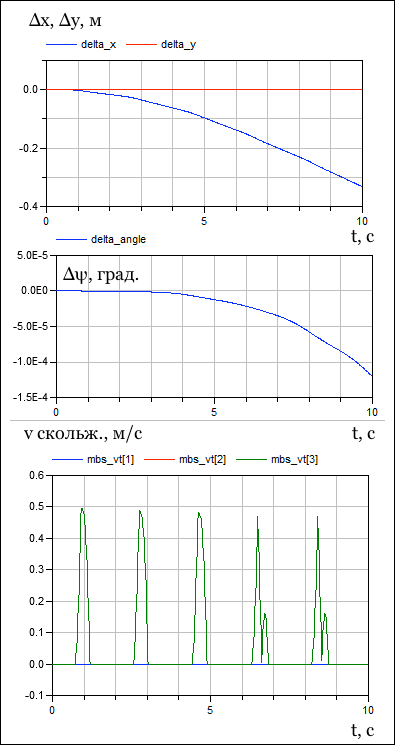
\includegraphics[width=7cm, viewport=0 0 395 745,clip]{content/parts/3_friction/diploma/img/res/comparison_v_1_0_omega_0_frac_1e-2_n_4_time_10s.png}\\
\eta = 0,1, v_0 = 1, \omega_0 = 0 & \eta = 0,01, v_0 = 1, \omega_0 = 0\\
\end{array}\end{equation*}\end{center}
\caption{Вращение экипажа с трением по прямой}
\end{figure}
\newpage

\begin{figure}[h]
\begin{center}\begin{equation*}\begin{array}{cc}
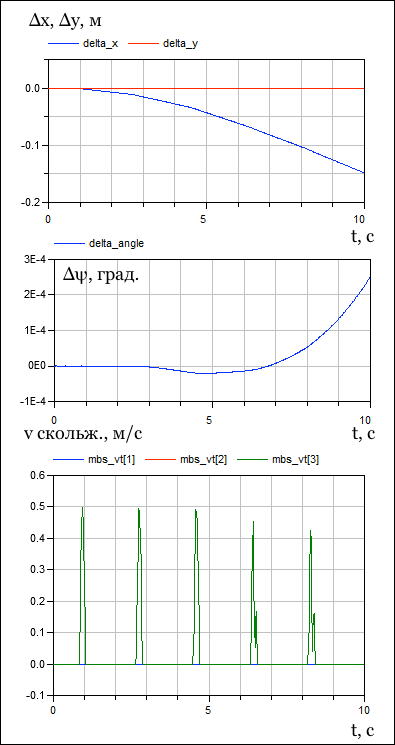
\includegraphics[width=7cm, viewport=0 0 395 745,clip]{content/parts/3_friction/diploma/img/res/comparison_v_1_0_omega_0_frac_1e-3_n_4_time_10s.png} & 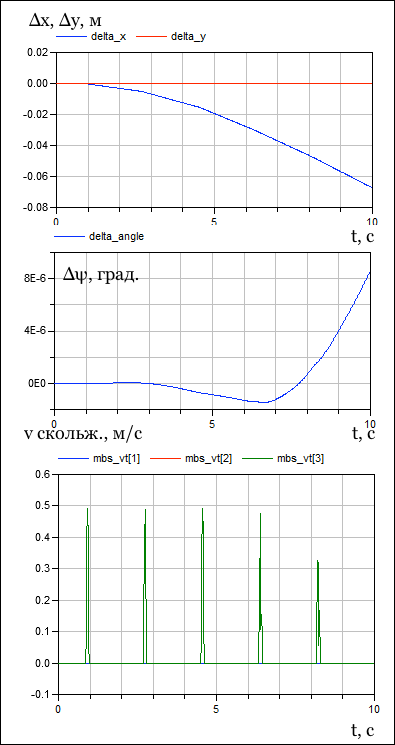
\includegraphics[width=7cm, viewport=0 0 395 745,clip]{content/parts/3_friction/diploma/img/res/comparison_v_1_0_omega_0_frac_1e-4_n_4_time_10s.png}\\
\eta = 0,001, v_0 = 1, \omega_0 = 0 & \eta = 0,0001, v_0 = 1, \omega_0 = 0\\
\end{array}\end{equation*}\end{center}
\caption{Вращение экипажа с трением по прямой}
\end{figure}
\newpage
